\documentclass[letterpaper, 10pt, conference]{IEEEtran}

\usepackage{amsmath,amsfonts}
\usepackage{algorithmic}
\usepackage{algorithm}
\usepackage{array}
\usepackage[caption=false,font=normalsize,labelfont=sf,textfont=sf]{subfig}
\usepackage{textcomp}
\usepackage{stfloats}
\usepackage{url}
\usepackage{verbatim}
\usepackage{graphicx}
\graphicspath{{../../}{../}}
\usepackage{booktabs}
% \usepackage{caption}
\usepackage{hyperref}

% \pdfinfo{
% /Author ()
% /Title ()
% /Creator ()
% }
\usepackage{cite}
\usepackage{float}
\usepackage[colorinlistoftodos]{todonotes}

\IEEEoverridecommandlockouts

    \title{\LARGE \bf
    Discovering of Gverning Equations DMD and SinDy for Nonlinear Physicla System The Kinetics Sculpture}

    \author{
    \IEEEauthorblockN{Justice V.~Essuman, Alhamduhaha Boker, Leonard Smith}
    \IEEEauthorblockA{Department of Electrical and Computer Engineering, Virginia Tech, Blacksburg, VA, USA\\
    justiceve@vt.edu, bokerece@vt.edu, lsmith@vt.edu}
    }

\begin{document}
    
    \maketitle
    \thispagestyle{empty}
    \pagestyle{empty}

    
%%%%%%%%%%%%%%%%%%%%%%%%%%%%%%%%%%%%%%%%%%%%%%%%%%%%%%%%%%%%%%%%%%%%%%%%%%%%%%%%
    \begin{abstract}
        The Swinging Sticks, a double-pendulum kinetic sculpture, represents a canonical example of nonlinear dynamics with strong sensitivity to initial conditions and complex energy transfer between coupled arms. Traditional physics-based models derived from Lagrangian mechanics capture their qualitative behavior but remain analytically intractable and highly sensitive to noise in experimental data.Following publishing of dataset of the kinectic sytsem
    \end{abstract}

    \begin{IEEEkeywords}
    Chaotic System, Dynamical System, Nonlinear System, Attractor, Hough Transform, Machine Learning
    \end{IEEEkeywords}

%%%%%%%%%%%%%%%%%%%%%%%%%%%%%%%%%%%%%%%%%%%%%%%%%%%%%%%%%%%%%%%%%%%%%%%%%%%%%%%%
    \section{Introduction and Motivation}
    
        The Swinging Sticks sculpture is an engineered double pendulum system designed to resemble a perpetual motion machine. From the popular scene in Iron Man 2 movie, like the double pendulum, its behavior has long fascinated physicists and engineers, inspiring the exploration of even more complex systems in nature: three body problems and chaos in physical systems. Its motion is sustained by sensors and magnets, yet the underlying physics is that of two coupled pendulums with very low damping \cite{noauthor_swinging_2022}. Multidegree-of-freedom pendulums, from the classic double pendulum up to higher arms-systems form the traditional examples of nonlinear dynamical systems. These systems exhibit a wide range of behavior, from simple harmonic oscillations at low energy, unpredictable oscillations or aperiodic trajectories to fully chaotic motion at higher energy levels \cite{kaheman_experimental_2022}. In particular, increasingly minute variations in initial angles lead to completely different trajectories: the swinging kinetic system, like the double-pendulum's motion, is famously chaotic, with strong sensitivity to initial conditions, posing a huge challenge to its predictability. There is also the importance of accounting for energy dissipation and external forces to avoid unrealistic predictions, an additional layer of complexity to the dynamics of the problem of this system. Adding more links increases complexity; multi-arm pendulums develop intricate phase-space structures that mediate transitions between different oscillation modes. These similar features in the swinging kinetic sticks make it challenging as benchmark for nonlinear dynamics and control studies.

        \begin{figure}[!t]
            \centering
            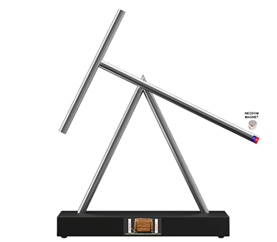
\includegraphics[width=2in]{figures/sticks.png}
            \caption{The Swinging Kinetic Sticks}
            \label{sticks}
        \end{figure}
        
        Results from machine learning research indicates the community lacks benchmarks for chaotic systems from real chaotic physical systems, which can be leveraged to test the reliability of predictive models. An accurate and adaptive model is required to fully understand the dynamics of the Swinging Kinetic system, as, unlike a simple double-pendulum system, the equations that govern the dynamics of its behavior are unknown. In this paper, an ablation study on time series prediction is performed using the top five best-performing time series predictor models from the literature on a novel dataset from the Swinging Kinetic Sculpture. Post identification of best model predictor, Dynamic Mode Decomposition (DMD) and Sparse Identification of Nonlinear Dynamics (SINDy) are proposed to be leveraged for the development of data-driven models for discovering the governing dynamics or equations of the Kinetic Swinging Sculpture.
        
%%%%%%%%%%%%%%%%%%%%%%%%%%%%%%%%%%%%%%%%%%%%%%%%%%%%%%%%%%%%%%%%%%%%%%%%%%%%%%%%
        \subsection{Related Works}    
            Classical approaches for discovering the dynamics of similar coupled systems is the Lagrangian or Hamiltonian formalisms. By choosing the limb angles as generated coordinates, one can derive the coupled nonlinear equations of motion from first principles \cite{noauthor_double_2025}. As such, the double pendulum Lagrangian is given by the kinetic minus the potential energy in terms of the two angles, leading to coupled second-order ODEs for the angles. These equations capture energy conservation and the full nonlinear coupling, but admit closed-form solutions only in special limits; small-angle approximations. In practice, analytical perturbation or numerical integration of these ODEs is used to understand mode shapes and energy transfer in the pendulum system, demonstrating effectiveness, but often being computationally intensive to tune for accuracy. Pendulum systems are known for their chaotic behavior as they exhibit bifurcation. In such models, the pendulum arms are abstracted into coupled oscillators, while torques are applied as input to control angular positions and velocities. The model effectively captures the effect of total kinetic energy on the phase space. 
    
            Koopman/DMD-based techniques take a different tack, embedding the nonlinear pendulum flow into a high-dimensional linear system. Applied to Lorenz and Rossler chaotic systems, and even a double pendulum, HAVOK can separate the dynamics into a dominant linear part with intermittent forcing\cite{brunton_chaos_2017}. In practice, these often achieve strong predictive accuracy and generalization. For instance, Berrueta et al. (2020) demonstrated that a polynomial EDMD (extended DMD) model of a simulated double pendulum had the lowest average error across state-space among several regressors \cite{mauroy_experimental_2020}. However, such models yield only a linear surrogate of the dynamics (not explicit ODEs). By contrast, deep recurrent networks (RNN/LSTMS) can directly learn the time series with remarkable short-term accuracy. In one study, an LSTM model predicted the next 1.5s of a chaotic double-pendulum trajectory within a tight error bound, whereas a best-fit analytic model diverged in just 0.12s \cite{noauthor_lstm_2024}. The drawback is that these neural models are opaque “black boxes” that do not produce human-readable equations \cite{purnomo_sparse_2023}.
            
            For prediction, with the ideal embedding dimension determined, reconstruction and forecasting of a chosen model can be performed. By comparing predictions from real data to those from surrogate data, using Takens’s embedding in its application of dynamic reconstruction and nonlinear prediction techniques to laboratory-generated geophysical data, smith refines earlier methods of detecting low-dimensional chaos \cite{smith_identification_1992}, using this method in the challenging task of distinguishing between deterministic and stochastic behaviors in low-dimensional dynamic systems.
        
        \subsection{Contribution and Novelty}
        
            This section outlines the novel contributions of this work, including the data acquisition process for the continuous study of the seemingly non-terminating motion of the Swinging Kinetic Stick sculpture and the first ablation study on the prediction of timeseries from its timeseries. Below are other major contributions of this study:.
            \begin{itemize}
                \item Published the first dataset of the motion of the Swinging Kinetic Sculpture System
                \item Introduced an approach for studying the overall evolution of the system until termination
                \item Proposed method for discovering the dynamics and governing equation of the system
            \end{itemize}
        \begin{figure}[htb]
        \centering
            \subfloat[Frame 1]{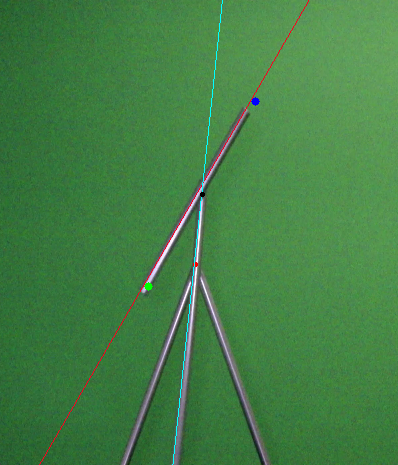
\includegraphics[width=0.2\textwidth]{figures/Frame 1.png}}\hfill
            \subfloat[Frame 2]{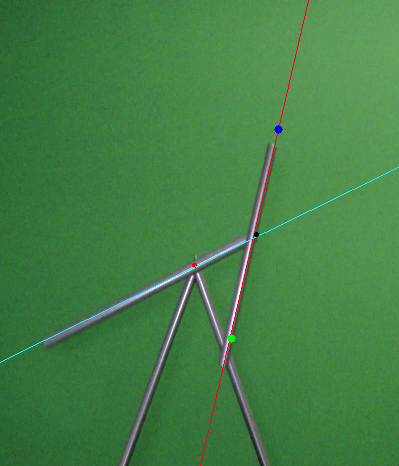
\includegraphics[width=0.2\textwidth]{figures/Frame 2.png}}\hfill
            \subfloat[Frame 3]{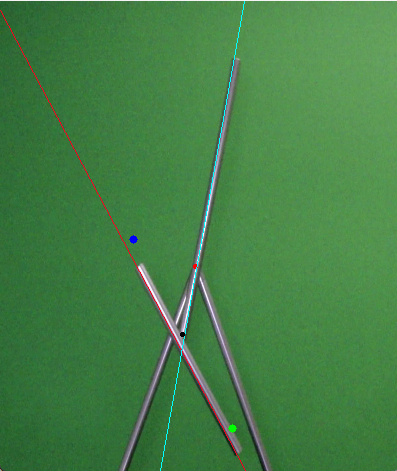
\includegraphics[width=0.2\textwidth]{figures/Frame 3.png}}... \hfill ...
            \subfloat[Frame n]{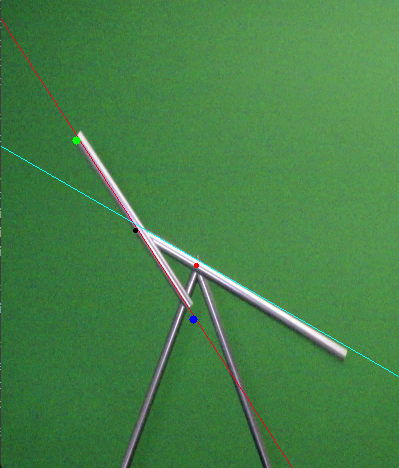
\includegraphics[width=0.2\textwidth]{figures/Frame 4.png}}
            \caption{A sequence of frames showing red line and green line tracking the motion of the short and long stick respectively. The red point is the center of the system. The blue and light green spots around the short stick serve as a guide for determining the short end of the short stick}
            \label{fig:four_frames_row}
        \end{figure}

        \subsection{Objective} 
            In this paper, the underlying behavior of the chaotic motion of swinging sticks is studied by predicting its next state from its timeseries and ultimately determining the best nonlinear model predictor ideal for timeseries prediction and forecasting of state of its dynamics. There is no known baseline best prediction model for reference on the predictability of swinging sticks timeseries. In the work, we seek to identify and establish this baseline for extended studies on this system.

        
    \section{The Swinging Kinetic System Chaotic Dataset}
        \subsection{Mechanical System}
            The swinging rods, also known as kinetic motion toys or kinetic sculptures, have captivated the imagination of both scientists and enthusiasts for decades. These mesmerizing contraptions consist of two (long and short) metallic rods(pendulums) connected by hinges that allow rotation. The system has a triangular support made up of stationary standing legs or edges with their meeting point serving as a center of rotation of the long rod.  The system is driven by an electromagnetic motor, driven by a magnetic field that initiates and sustains oscillations. The swinging rods have a powerful neodymium magnet in them that enables them to exhibit complex nonlinear dynamics due to their coupled motion and sensitivity to initial conditions. When set in motion, they exhibit complex rhythmic patterns, seemingly defying gravity as they gracefully swing and rotate. The dynamics governing the motion of these rods are not only fascinating from an aesthetic standpoint but also hold profound implications like every double pendulum system in physics, engineering, and mathematics with rich dynamic behavior. Exploring the underlying principles behind these dynamics not only enriches our understanding of mechanical systems, but also provides insights into broader scientific and technological domains. 
            
            \begin{figure}[htbp]
                \centering
                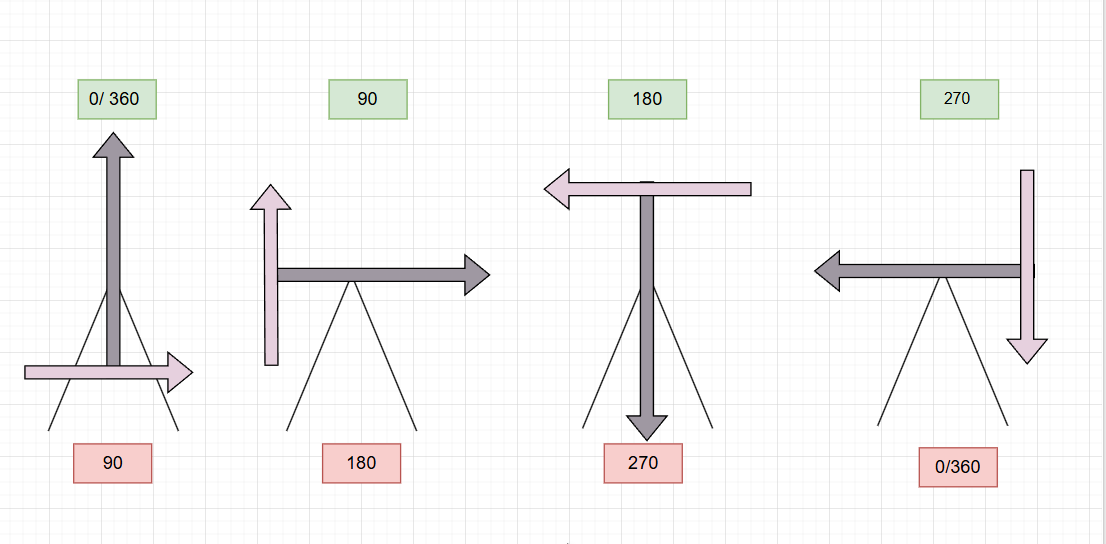
\includegraphics[width=1\columnwidth]{figures/sticks_configuration.png}
                \caption{The graph shows the orientation configuration used for tracking the evolution of motion of the short stick (angle in red) and long stick (angle in green) of the system. The longer end and the shorter ends of the long and short sticks, respectively served as their pointers}
                \label{fig:sticks_configuration}
            \end{figure}
            
            \begin{table}[htbp]
                \centering
                \caption{Camera settings.}
                \label{tab:camera_settings}
                \begin{tabular}{lr}
                    \hline
                    \multicolumn{2}{c}{\textbf{Camera settings}} \\
                    \hline
                    Focal length [mm] & 50 \\
                    Frame exposure time [\textmu s] & 90 \\
                    Capture frame-rate [FPS] & 60 \\
                    Image resolution [px] & 1920 $\times$ 1080 \\
                    \hline
                \end{tabular}
            \end{table}

        \subsection{Data Acquisition Process}
            
            The process involved using a high-quality camera and video recording the motion of the sticks with a resolution of 1920 x 1080 at 60 fps. The exposure of the lens was set high to allow light to be captured; hence the light setting was made normal and augment with an extra DC power LED to illuminate the room. To allow the easy extraction of the sticks position and to avoid shadow interference, a green screen background was used. For each of the measurements explained below, the system's initial condition on start involves displacement of the Swing sticks or rod, long and short, at 0° and 90°, respectively. The initial configurations defined from the angles of the sticks determined are shown in figure. 

        \subsection{Long and Short Arm Positions Extraction}
            The raw video was run through an OpenCV based image processing program that utilizes details like center of the frame, long stick perpendicular distance from the center to extract the positions and ultimately the angles of rotation of both long and short sticks.
            This is realized using the Hough transform detection of long and short rod's orientation via line detection. The Hough transform function outputs all straight lines detected in each frame in $\rho, \theta$ pairs, where $\rho$ is the perpendicular distance the lines make from the top left corner of the frame and $\theta$ is the angle the perpendicular to the lines makes with the horizontal frame. The  $\rho, \theta$  values were further used to determine the endpoints of the lines and their actual orientation using an algorithm in python which writes the angles of rotation of the long and short sticks into file.
        
            The timeseries data gathered from this system serves as data from a real-world system that we ultimately will test our improved forecasting models against. For this physical system, our interest in it as a chaotic system is the number of times the long stick crosses the top and also the equations of its dynamics. The preliminary results are presented in the results section however the algorithm is detailed below.
            
            \begin{figure}[htbp]
                \centering
                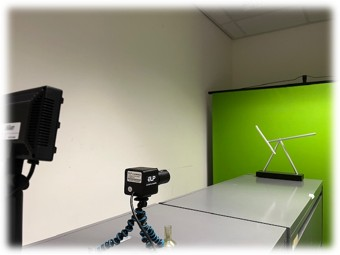
\includegraphics[width=\linewidth,  height=6cm, keepaspectratio]{figures/sticks_setup.jpg}
                \caption{Shows the hardware setup for the data acquisition process; with lamp stand, camera, the kinetic swinging sculpture and a green background to enable improved image processing}
                \label{fig:hardware_setup}
            \end{figure}
        

    \section{Methodology}
        
        \subsection{Experimental System and  Setup} 
            The first attempt at gathering data from such a chaotic physical system done in this section. The process resulted in two sets of times series data representing the rotation of the long and short sticks of the system. The experimental setup involved the following:

            \begin{itemize}
                \item \textit{The Kinetic Swing Sticks}:  A commercial kinetic energy system with two freely rotating sticks. 
                
                \item  \textit{Measurement Devices}: 
                    A high-resolution camera (60 fps or higher) is used to capture the motion of the system. The camera is positioned to record the side view ensuring that both the angular displacement and velocity of the rods are visible.
                    
                \item \textit{Data Acquisition System}: A Lenovo laptop is connected to the camera to collect data of the motion of the sticks in real. A text file is also used in collecting the data produced from the detection of rod motion detection algorithm.
            \end{itemize}

        \subsection{Image Processing Algorithm }
            \begin{algorithm}[ht]
                \caption{Sticks Angles Data Acquisition per Frame}
                \label{alg:sticks_detection_algorithm}
                \footnotesize
                    \begin{algorithmic}[1]
                    
                    \REQUIRE Recorded video (1920$\times$1080)
                    \ENSURE $long\_stick\_angle$, $short\_stick\_angle$
                    
                    \STATE Resize frame to 640$\times$480; set center $[320,340]$
                    \STATE Apply Hough transform to obtain $(\rho,\theta)$
                    \STATE Filter stands:
                           left $\theta \in [18^\circ,24^\circ]$,
                           right $\theta \in [155^\circ,163^\circ]$
                    \STATE Remove stand lines; retain stick lines
                    \STATE Group and average stick angles
                    \STATE Convert $(\rho,\theta)$ to Cartesian form
                    
                    \FOR{angle transitions in $[175^\circ,185^\circ]$}
                        \STATE Add $180^\circ$ for continuity
                    \ENDFOR
                    
                    \STATE Compute line equations:
                           $y=m_1x+b_1$, $y=m_2x+b_2$
                    \STATE Compute intersection:
                           \[
                           x_{poi}=\frac{b_2-b_1}{m_1-m_2},
                           \quad
                           y_{poi}=m_1x_{poi}+b_1
                           \]
                    
                    \RETURN $frame\_number$, $time$,
                            $long\_stick\_angle$,
                            $short\_stick\_angle, ott$
                    
                    \end{algorithmic}
                An elaborate version of the algorithm is provided in the appendix \ref{s:elaborate sticks algorithm}.
            \end{algorithm}
            

            \begin{figure}[ht]
                \centering
                
                \captionsetup[subfloat]{font=footnotesize}
                
                \subfloat[Frame]{%
                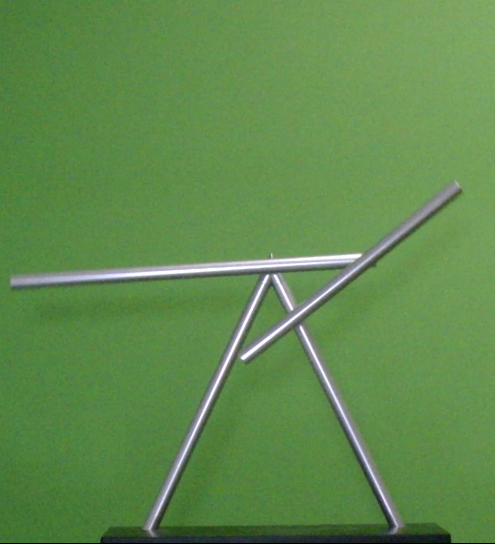
\includegraphics[width=0.3\columnwidth,
                                 height=0.35\columnwidth]
                {figures/image_stick2.png}}
                \hspace{0.005\columnwidth}
                \subfloat[Detection]{%
                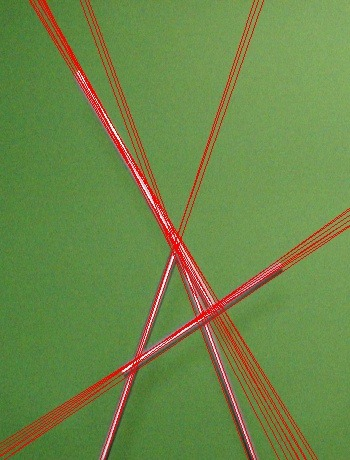
\includegraphics[width=0.3\columnwidth,
                                 height=0.35\columnwidth]
                {figures/hough_1.jpg}}
                \hspace{0.005\columnwidth}
                \subfloat[Tracking]{%
                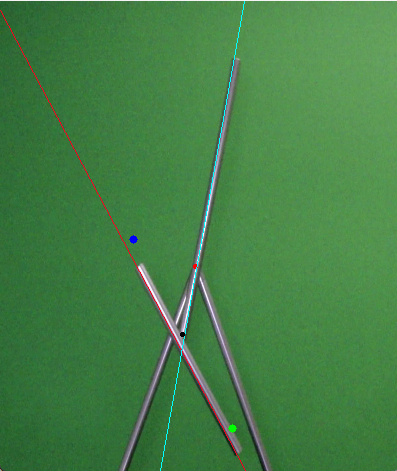
\includegraphics[width=0.3\columnwidth,
                                 height=0.35\columnwidth]
                {figures/Frame 3.png}}
                
                \caption{These frames show the major stages of the angle position acquisition algorithm which processes angle positions of short and long sticks frame by frame. For each frame(a), hough transform detects lines which are grouped and ultimately tracked frame by frame }
                \label{fig:stages_of_algorithm}
        \end{figure}
        
        \subsection{Data Cleaning  and Smoothening}
            Considering the rotation of the angles is sinusoidal in nature a quadratic polynomial smoothening technique would be ideal for the smoothening process. This is verified by comparing the quadratic polynomial fit against linear fit for the pure sine wave, noisy sine wave and sticks long angle. 
            For the smoothing process, a sliding window approach is adopted with a window size of 11 applied to a 60-frames-per-second time series consisting of 60 angle measurements. The fit is performed on each set of 11 consecutive angles, after which the window is shifted by one step. This process is repeated until all angles are processed. This produces a distribution of fitted values for each angle, with the first and last angles being fitted only once. The results show that linear fits exhibit a higher residual range and perform overall worse compared to quadratic fits, which closely approximate the true values. The method was subsequently tested on actual stick data, with results shown in \autoref{fig:cleaning} and \autoref{fig:short_long_sticks_clean}. Throughout these plots, the angles are also referred to as observed values. Gaussian noise with a standard deviation of 5 is added.

            
            \begin{figure}[ht]
                \centering
                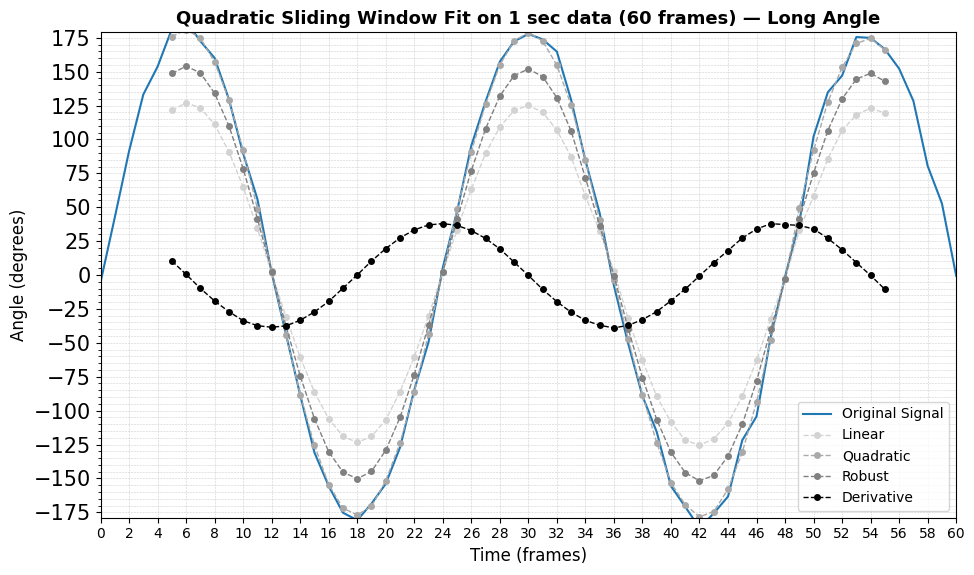
\includegraphics[width=1 \linewidth]{figures/quadratic_smoothening.png}
                \centering
            \caption{The graphs illustrates the choice of robust sliding window quadratic smoothening technique for removing data fluctuation. Cleaning of data is performed on 60 frames of data from the long and short stick motion}
                \label{fig:cleaning}
            \end{figure}

         \subsection{Data Generation}
            The timeseries of the long and short sticks were generated from the system with an initial condition of long stick displacement angle of 90 degrees while the short stick remained at rest. A fifteen hours and twenty hours continuous data data acquisition process produced 3 million and 5 million data points respectively. The resulting time series used for this ablation study has $N=3000$ points. Total series length of $N=3000$ is consistent with the literature used for Ikeda ~\cite{jaeger_harnessing_2004, pathak_model-free_2018}.
        
        \subsection{Embedding and Feature Construction}
            Supervised input-output pairs were constructed via Takens'
            delay embedding theorem~\cite{rand_detecting_1981-2}:
            with embedding dimension $d=5$ and delay $\tau=1$. All inputs and
            outputs were standardized to zero mean and unit variance.

            $N_{\mathrm{train}}=2000$ consecutive samples were used for training
            (ordered in time; no shuffling to preserve dynamical structure), followed
            by $N_{\mathrm{test}}=1000$ for evaluation. This 2:1 ratio follows
            standard practice in chaotic benchmark studies.

        \begin{figure}[ht]
                \centering
                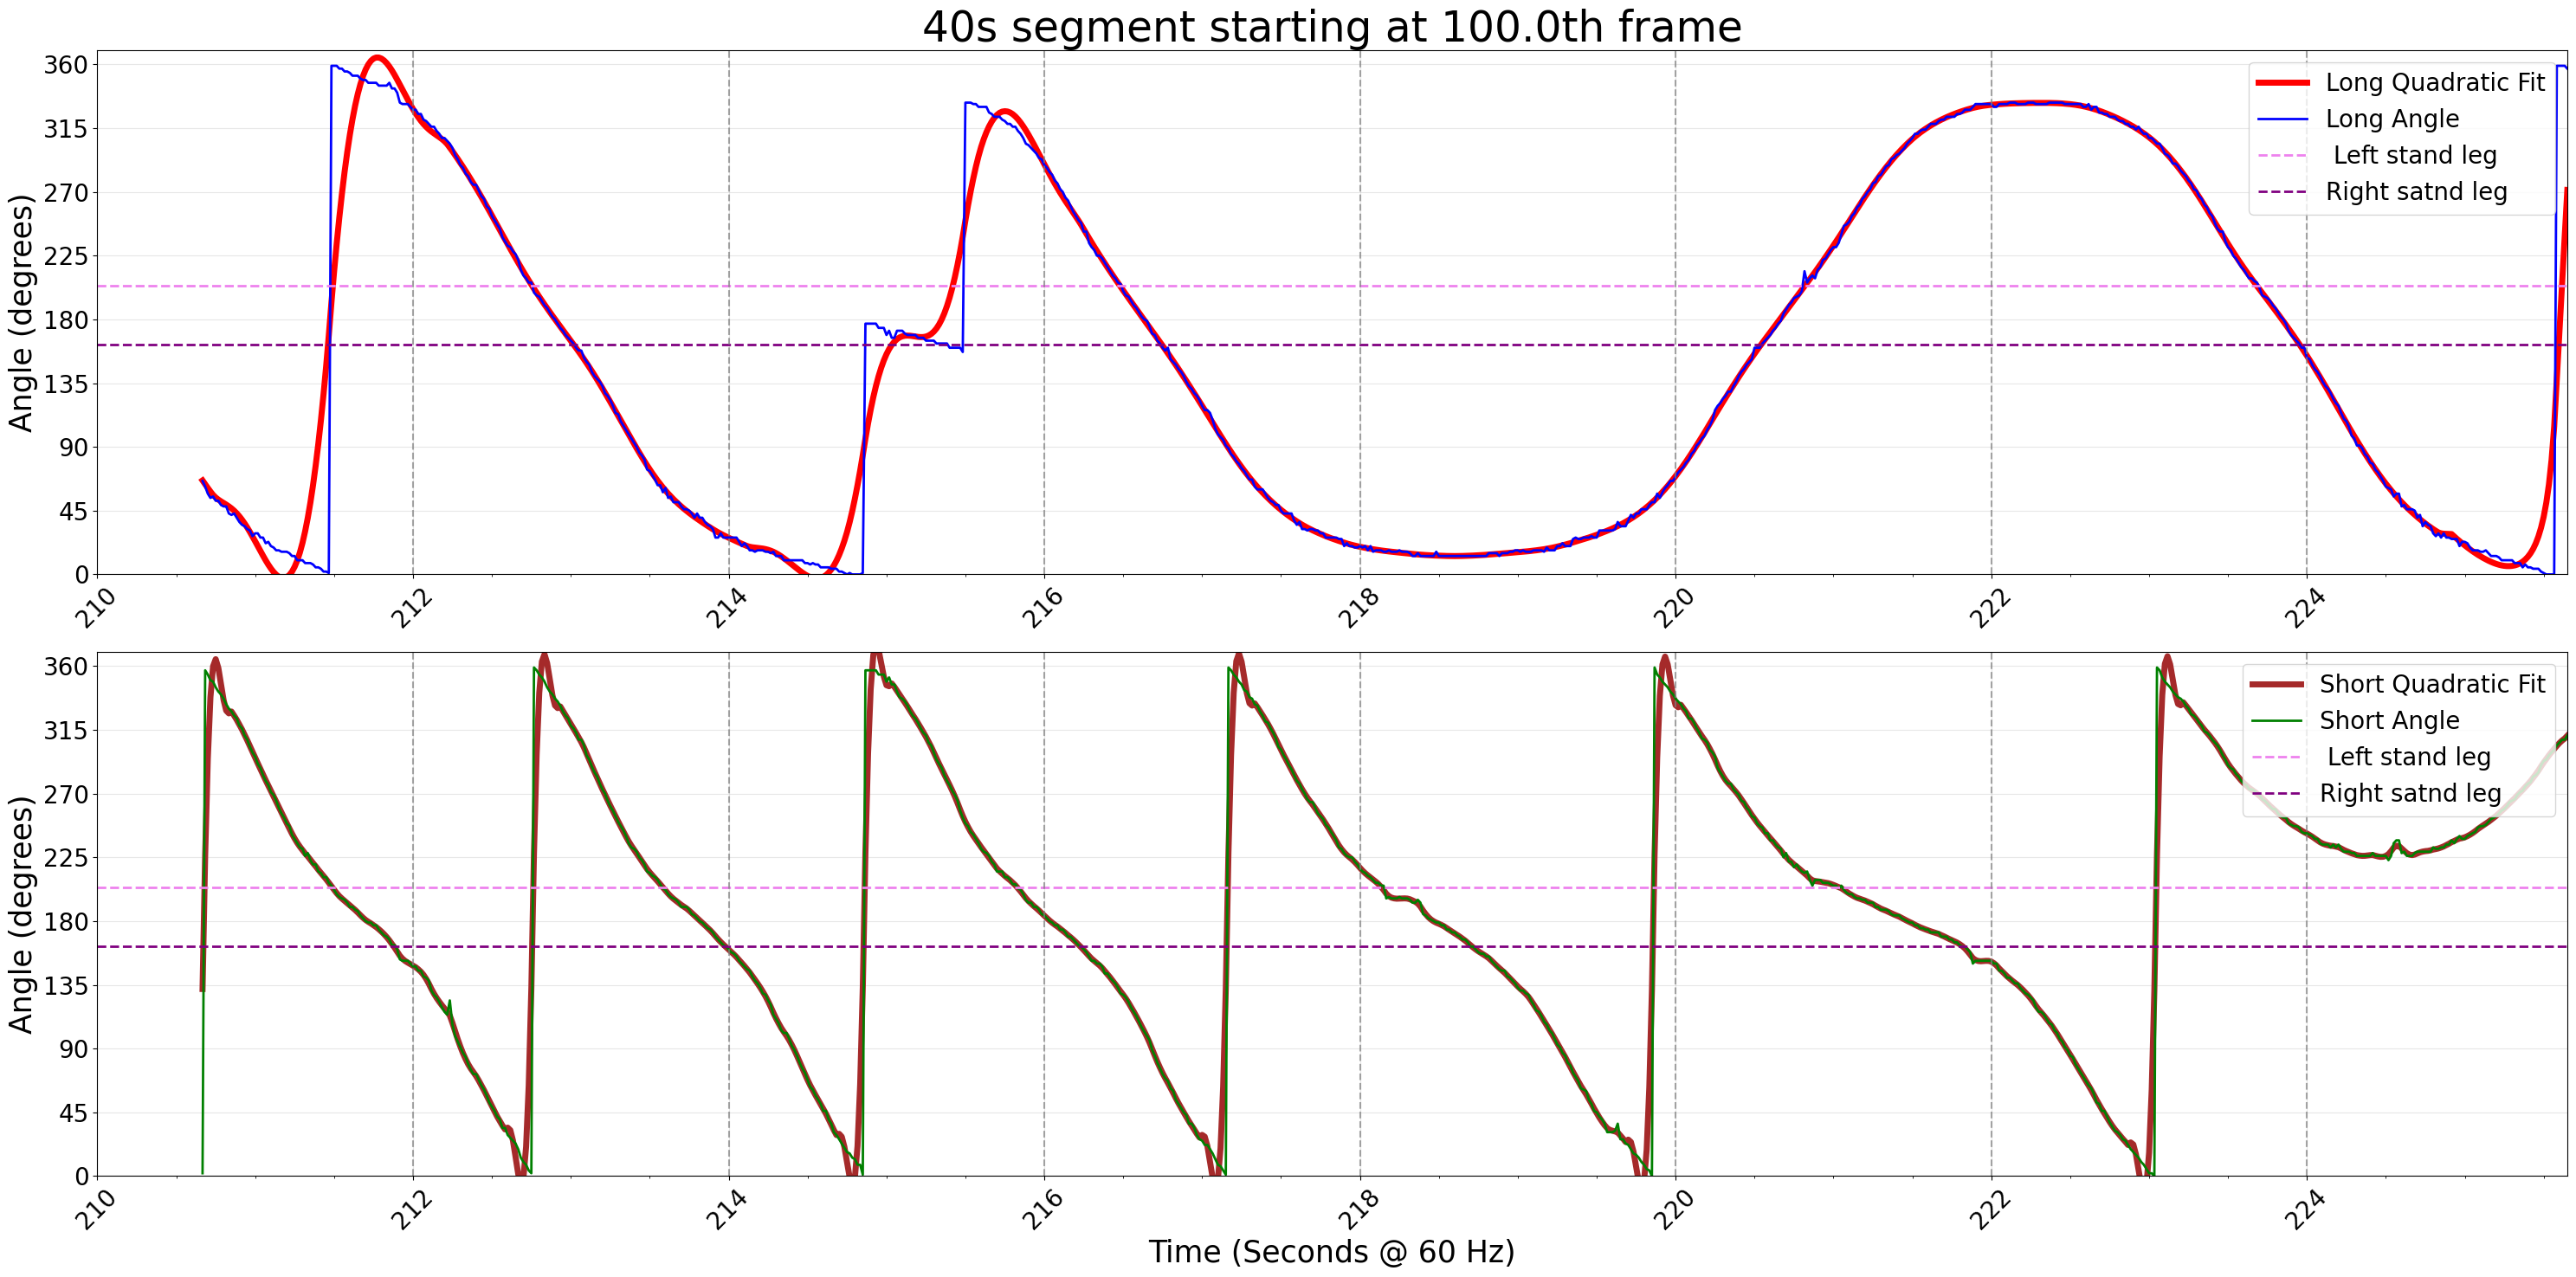
\includegraphics[width=1 \linewidth]{figures/long_short_sticks_raw_n_cleaned.png}
                \centering
                \caption{The graph on the top shows a section of raw(blue) and cleaned(red) of long stick timeseries. The bottom graph shows the raw(brown) and cleaned (green) timeseries of the short stick. The dotted lines on both graphs show the position of the left and right stands of the system}
                \label{fig:short_long_sticks_clean}
        \end{figure}
    
\subsection{\textbf{Circular Delay Embedding for the Angular State Evolution}}
\label{ssec:circular_embedding}

    The stick angle $\theta$ recorded by the tracking algorithm of in the appenedix is not a general scalar; not just a monotonously increasing or decreasing
    % Section  is not a generic scalar
    value: it is an element of the circle $\theta \in [0^{\circ},360^{\circ})$
    with the identification $0^{\circ}\equiv 360^{\circ}$, i.e.\ a point of
    $\mathbb{R}/360^{\circ}, S^1$. %\mathbb{Z} \cong S^1 
    The delay-embedding construction
    of from Takens' Section %~\ref{ssec:embedding} 
    builds, at every time index $i$, a vector of
    $d$ lagged observations separated by delay $\tau$,
    \begin{equation}
        \mathbf{v}_i = \bigl[\theta_i,\ \theta_{i-\tau},\ \theta_{i-2\tau},\ \dots,\ \theta_{i-(d-1)\tau}\bigr],
        \label{eq:raw_delay_vector}
    \end{equation}
    which the local-linear predictor (Section~\ref{sssec:regression_recovery}) uses both to
    search for analogue states and as the model for
    $\widehat{x}_{t+1}\approx\mathbf{A}\mathbf{x}_t+\mathbf{b}$. At the core or fundamental stage of this algorithm hinges on one further goal: a notion of distance between two
    delay vectors, used to select the $k$ nearest neighbours the local-linear
    fit is built from. We first show that the distance used in our old
    embedding representation is the wrong metric for studying or predicting the dynamics of a periodic kinetic swinging system, and then give the
    embedding under which it becomes the correct one. \\

    \subsubsection{Baseline: Euclidean Distance on Raw-Degree Vectors}
    \label{sssec:raw_distance}

        Nearest-neighbour search over the training set
        $\{\mathbf{v}_j\}_{j=1}^{N_{\mathrm{train}}}$ is performed with a
        kD-tree,  %(\texttt{scipy.spatial.cKDTree}), 
        which indexes points in $\mathbb{R}^d$ and answers a query $\mathbf{v}_i$ by returning the
        $k$ training vectors minimising the Minkowski-$p$ distance, with
        $p=2$ (2-norm) as the default. Time indices are excluded from the indexed
        coordinates, so the KD-tree operates purely on the $d$ lagged
        angle values, and the distance between two raw delay vectors
        $\mathbf{v}_i,\mathbf{v}_j\in\mathbb{R}^d$ is
        \begin{equation}
            d_{\mathrm{raw}}(\mathbf{v}_i,\mathbf{v}_j)
                = \left(\sum_{l=0}^{d-1}\bigl(\theta_i^{(l)}-\theta_j^{(l)}\bigr)^2\right)^{\!1/2}.
            \label{eq:raw_distance}
        \end{equation}

        Equation~\eqref{eq:raw_distance} is the correct metric on
        $\mathbb{R}^d$, but the coordinates $\theta^{(l)}$ do not live in
        $\mathbb{R}^d$: each lies on $S^1$, and~\eqref{eq:raw_distance}
        silently treats $S^1$ as if it were cut open into the interval
        $[0^{\circ},360^{\circ})$ and laid flat on the real line. That cut
        introduces a discontinuity exactly where none exists physically. Take
        a query angle $\theta_i = 349^{\circ}$ as the last current state in  delay vector against two library candidates delay vectors with last vector values
        $\theta_A = 5^{\circ}$ and $\theta_B = 200^{\circ}$. The true angular
        separations, measured the short way around the circle, are
        $16^{\circ}$ ($\theta_i$ to $\theta_A$) and $149^{\circ}$ ($\theta_i$
        to $\theta_B$) -- $A$ is by far the closer point. Equation~\eqref{eq:raw_distance},
        evaluated on the open interval, gives instead
        $|349^{\circ}-5^{\circ}| = 344^{\circ}$ and
        $|349^{\circ}-200^{\circ}| = 149^{\circ}$: the KD-tree ranks $B$ as
        the nearer neighbour, the opposite of the physical ordering. Every
        delay window whose lags straddle the $0^{\circ}/360^{\circ}$ boundary
        is subject to this misranking, which is not a rare edge case for a
        system whose long stick completes full revolutions or over the top crossings.

        The error does not stop at neighbour selection. Even a distance
        metric that correctly ranked neighbours near the wrap (e.g.\ a
        periodickD tree) would leave the regression step in
        error, because the local-linear fit $\mathbf{A}\mathbf{x}_t+\mathbf{b}$
        is estimated by ordinary least squares over the $k$ neighbour
        targets. A neighbourhood of angles genuinely clustered near the wrap,
        e.g.\ $\{358^{\circ},\,2^{\circ},\,359^{\circ},\,1^{\circ}\}$, is
        clustered near $0^{\circ}$ physically, but its arithmetic mean under
        \eqref{eq:raw_delay_vector}'s flat-interval representation is
        $\approx180^{\circ}$, utterly wrong. Ordinary least squares
        computes exactly such an arithmetic average implicitly; the raw-degree
        representation therefore corrupts the target space represnetation of the regression
        independently of how the neighbors were found. This second effect is
        the reason the fix below changes the representation itself rather
        than only the distance function used for the kD tree search. \\

    \subsubsection{Improved Representation: Embedding onto the Unit Circle} 
    \label{sssec:circular_distance}


        The standard remedy in directional statistics %~\cite{mardia_directional_1999}
        for placing an angular variable into a Euclidean space without
        introducing a cut point is the embedding
        \begin{equation}
            \Phi:\ \theta \ \longmapsto\ (\cos\theta,\ \sin\theta)\ \in\ S^1\subset\mathbb{R}^2,
            \label{eq:unit_circle_map}
        \end{equation}
        which is continuous and injective on $[0^{\circ},360^{\circ})$, so no
        two physically distinct angles are ever identified, and no boundary
        is introduced where none exists. Applying $\Phi$ to every lag of
        \eqref{eq:raw_delay_vector} in place of the raw angle gives the
        \emph{circular delay vector}
        \begin{equation}
            \widetilde{\mathbf{v}}_i = \bigl[\cos\theta_i^{(l)},\ \sin\theta_i^{(l)}\bigr]_{l=0}^{d-1} \in \mathbb{R}^{2d},
                \qquad \theta_i^{(l)} := \theta_{i-l\tau},
            \label{eq:circular_delay_vector}
        \end{equation}
        i.e.\ every lag doubles from one raw-degree coordinate to a
        $(\cos,\sin)$ pair, and the kD tree is built over this $2d$-dimensional
        space instead, \emph{the search algorithm itself is unchanged}; only
        the geometry of the space it searches is corrected.

        The Euclidean distance between two points on the image of $\Phi$
        reduces to a closed form. For two angles $\theta_i,\theta_j$,
        \begin{align}
            \bigl\|\Phi(\theta_i)-\Phi(\theta_j)\bigr\|_2^2
                &= (\cos\theta_i-\cos\theta_j)^2 + (\sin\theta_i-\sin\theta_j)^2 \notag\\
                &= 2 - 2\cos(\theta_i-\theta_j) \notag\\
                &= 4\sin^2\!\left(\tfrac{\theta_i-\theta_j}{2}\right),
            \label{eq:chord_derivation}
        \end{align}
        using $\cos(a-b)=\cos a\cos b+\sin a\sin b$ and the half-angle
        identity $1-\cos x = 2\sin^2(x/2)$. Hence
        \begin{equation}
            d_{\mathrm{chord}}(\theta_i,\theta_j)\ :=\ \bigl\|\Phi(\theta_i)-\Phi(\theta_j)\bigr\|_2
                = 2\left|\sin\!\left(\frac{\theta_i-\theta_j}{2}\right)\right|,
            \label{eq:chord_distance}
        \end{equation}
        the \emph{chord distance} on the unit circle. Unlike
        \eqref{eq:raw_distance}, $d_{\mathrm{chord}}$ is a strictly increasing
        function of the true angular separation
        $\Delta\theta = \min\bigl(|\theta_i-\theta_j|,\ 360^{\circ}-|\theta_i-\theta_j|\bigr)\in[0^{\circ},180^{\circ}]$,
        so ranking candidates by \eqref{eq:chord_distance} is equivalent to
        ranking them by physical closeness on the circle, with no
        discontinuity at $0^{\circ}/360^{\circ}$: $d_{\mathrm{chord}}$ is bounded
        in $[0,2]$ and attains its maximum only at the true antipode
        $\Delta\theta=180^{\circ}$. Summed over the $d$ lags, the distance
        between two circular delay vectors is
        \begin{equation}
            d_{\mathrm{circ}}(\widetilde{\mathbf{v}}_i,\widetilde{\mathbf{v}}_j)
                = \left(\sum_{l=0}^{d-1} 4\sin^2\!\left(\frac{\theta_i^{(l)}-\theta_j^{(l)}}{2}\right)\right)^{\!1/2},
            \label{eq:circ_distance_full}
        \end{equation}
        which is again an ordinary $\ell_2$ norm -- now correctly applied,
        since it is computed in the ambient Euclidean space $\mathbb{R}^{2d}$
        that $S^1\times\cdots\times S^1$ is embedded in, rather than in the
        periodic space itself.

        Re-evaluating the worked example of
        Section~\ref{sssec:raw_distance} under \eqref{eq:chord_distance}:
        $d_{\mathrm{chord}}(349^{\circ},5^{\circ}) = 2\sin(8^{\circ}) = 0.28$
        and $d_{\mathrm{chord}}(349^{\circ},200^{\circ}) = 2\sin(74.5^{\circ}) = 1.93$.
        ThekD tree now correctly ranks $A$ as the nearer neighbour
        ($0.28 < 1.93$), matching the true $16^{\circ}$ versus $149^{\circ}$
        angular separations.

    \subsubsection{Regression and Forecast Recovery}
    \label{sssec:regression_recovery}

        With neighbours selected under \eqref{eq:circ_distance_full}, the
        local-linear model is fit jointly on the two-dimensional target
        $\mathbf{y}=(\cos\theta,\sin\theta)$ rather than on the raw angle,
        \begin{equation}
            \widehat{\mathbf{y}}_{t+1} \approx \mathbf{A}\mathbf{x}_t+\mathbf{b},
            \qquad \mathbf{A}\in\mathbb{R}^{2\times 2d},\ \mathbf{b}\in\mathbb{R}^{2},
            \label{eq:circ_local_linear}
        \end{equation}
        by ridge-regularised least squares over the same $k$ neighbours, and
        the forecast angle is recovered by
        \begin{equation}
            \widehat{\theta}_{t+1} = \operatorname{atan2}\!\bigl(\widehat{y}_{t+1},\widehat{x}_{t+1}\bigr)\ \bmod\ 360^{\circ}.
            \label{eq:atan2_recovery}
        \end{equation}
        Because $\operatorname{atan2}$ is defined for every
        $(\widehat{x}_{t+1},\widehat{y}_{t+1})\neq(0,0)$,
        \eqref{eq:atan2_recovery} always returns a valid angle in
        $[0^{\circ},360^{\circ})$ with no clamping of the model output --
        under the raw-degree representation of Section~\ref{sssec:raw_distance},
        by contrast, the unconstrained regression output can and does fall
        outside $[0^{\circ},360^{\circ})$ whenever a neighbourhood spans the
        wrap, which is the direct mechanism behind the largest observed
        errors under that baseline (Section~\ref{sssec:circ_results}). The
        residual magnitude $r=\sqrt{\widehat{x}_{t+1}^{\,2}+\widehat{y}_{t+1}^{\,2}}$
        is a byproduct of \eqref{eq:circ_local_linear} with no counterpart in
        the raw-degree pipeline: $r\approx 1$ indicates the $k$ neighbours
        agreed closely on a forecast direction, while $r\to 0$ flags a
        neighbourhood whose targets pointed in conflicting directions, for
        which $\widehat{\theta}_{t+1}$ is correspondingly ill-conditioned.
        Forecast error itself is scored with the matching wrap-aware
        quantity,
        \begin{equation}
            e = \bigl((\widehat{\theta}_{t+1}-\theta_{t+1}) + 180^{\circ}\bigr) \bmod 360^{\circ} - 180^{\circ},
            \label{eq:circular_error}
        \end{equation}
        bounded to $(-180^{\circ},180^{\circ}]$, so that a $359^{\circ}$
        prediction against a $1^{\circ}$ target scores as the physically
        correct $2^{\circ}$ error rather than $358^{\circ}$.

    \subsubsection{Empirical Comparison}
    \label{sssec:circ_results}

        Table~\ref{tab:circular_comparison} compares the two embeddings on
        the long-stick series (60\,fps source, decimated to $\Delta t=0.5$\,s,
        $d=5$, $\tau=3$ steps ($1.5$\,s), forecast horizon $3$ steps ($1.5$\,s
        ahead), $k=16$), holding the local-linear predictor, the delay
        parameters, and the temporal train/test split identical across rows.
        Error is reported under the common circular metric
        \eqref{eq:circular_error} in both rows, so that the raw-degree
        embedding's own error column is not inflated relative to the
        circular embedding's by definition. The circular embedding at
        $N_{\mathrm{train}}=1024$ outperforms the raw-degree embedding even
        at $N_{\mathrm{train}}=4096$, indicating that at this lead time the
        state-space representation, not the size of the training library, is
        the binding constraint on forecast skill.

        \begin{table}[htbp]
        \begin{center}
        \caption{Long-stick forecast error by delay-vector representation, evaluated under the common wrap-aware error \eqref{eq:circular_error}. $d=5$, $\tau=3$ steps ($1.5$\,s), horizon $=3$ steps ($1.5$\,s ahead), $k=16$, $N_{\mathrm{test}}=2000$.}
        \label{tab:circular_comparison}
        \begin{tabular}{|l|r|r|r|}
        \hline
        \textbf{Embedding} & \textbf{$N_{\mathrm{train}}$} & \textbf{RMSE ($^\circ$)} & \textbf{MAE ($^\circ$)} \\ \hline
        Raw-degree, $\mathbb{R}^{d}$    & 1024 & 83.9 & 66.5 \\ \hline
        Raw-degree, $\mathbb{R}^{d}$    & 4096 & 72.3 & 53.3 \\ \hline
        Circular, $\mathbb{R}^{2d}$     & 1024 & \textbf{65.1} & \textbf{46.0} \\ \hline
        \end{tabular}
        \end{center}
        \end{table}

        Beyond the aggregate error reduction, the raw-degree embedding's
        largest errors are structurally different in kind from the circular
        embedding's: because the raw-degree regression output is
        unconstrained, its worst-case errors exceed $360^{\circ}$ in
        magnitude on this dataset, a signature of the mechanism described in
        Section~\ref{sssec:regression_recovery} rather than of ordinary
        forecast difficulty. The circular embedding's error is bounded by
        construction to $180^{\circ}$ regardless of how poorly a given
        neighbourhood agrees, since \eqref{eq:atan2_recovery} cannot produce
        an angle outside $[0^{\circ},360^{\circ})$. The remaining error at
        $65^{\circ}$--$84^{\circ}$ RMSE is not attributable to the
        representation: it is close to uniform across the swing (not
        concentrated at the sharp reversals near the top and bottom of each
        oscillation, nor correlated with local angular speed), consistent
        instead with a forecast horizon that is an appreciable fraction of
        the system's natural swing period, and with the embedding being
        univariate in the long-stick angle alone despite the coupled,
        two-arm nature of the physical system.



       
    
        \section{Mechanical Model and Coordinates}
            \begin{figure}[ht]
                \centering
                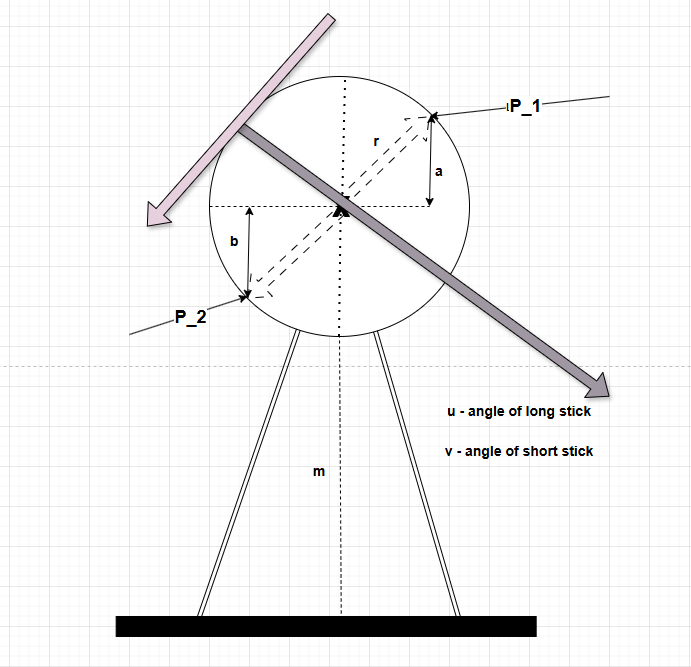
\includegraphics[width=3in]{figures/angle_config.png}
                \caption{Coordinates and Parameter of interest of the the Swinging Kinetic Sticks mechanical system. $r$ is the axis of rotation of the long stick and $e$ for nonstationary axis of rotation of the short stick}
                \label{fig:angle_config}
                    \end{figure}
                 In this section, the process for turning simultaneous angular position and angular velocity timeseries of the two sticks(rods) into their corresponding Potential Energy $U(t)$, Kinetic Energy $V(t)$ and Total angular momentum $L(t)$. 
            
                 The system dynamics of the system can be modeled first as two rigid uniform rods rotating about a single fixed axis. The long rod (angle $\theta_L$) and the short rod (angle $\theta_S$) each have one rotational degree of freedom; they are coupled only through the near-hub neodymium magnets. By simplifying the system and considering short stick as having same axis of rotation for the long stick( at point $P_1$) and short stick(reaching reached $P_2$), each rotating independently in one plane, magnetically coupled at the central axis of rotation $O$. Assume short stick has not coupled to long and determine it potential energy later the axis of rotation of the shorter stick can be later treated as non-stationary. 

                 System coordinates: $q = (\theta_L,\ \theta_S)$.

                 The tracked angle is in degrees, zero pointing up, increasing clockwise or decreasing counter-clockwise. For mechanics we want radians and a right-handed convention. Define, per rod,

                 \begin{align}
                     \varphi_i(t) \;=\; \varphi_i^{0} \;-\; \frac{\pi}{180}\,\theta_i^{\text{clean}}(t),
                     \qquad i \in \{L, S\}
                 \end{align}

                 To determine the kinetic and potential energy of each of the sticks, for each stick in pure rotation motion, calculate the following:.
                \subsubsection{Center of Mass Position (CM)}
                    \begin{align}
                        y_{\mathrm{cm},i}(t) = y_0 + d_i\cos\beta_i(t), 
                    \end{align}
                    where $\beta_i(t) = \varphi_i^{\text{s}}(t) + \gamma_i$ is the angle of the CM position vector from the upward vertical, and $\gamma_i \in \{0,\pi\}$ accounts for the CM lying on the pointer side of $O$. $y_O$ is an arbitrary initial or starting point of CM and abstracting out of all dynamics.
                
                \subsubsection{\textbf{Angular Velocity}}
                    Using the unwrapped version of the angle yields a continuous function suitable for differentiation. However using the timeseries which have already been de-noised and quadratically smoothened will still be wrapped. Apply differentiation will amplify high-frequency noise, so apply Savitzky-Golar filter %(using polynomial order $p=3$, window $W \approx 9\text{–}15$ samples $\approx 0.15\text{–}0.25$s)

                    \begin{align}
                        \varphi_i &= \mathrm{SG}\!\left(\varphi_i,\, W,\, p,\, \text{deriv}=0\right), \\
                        \omega_i = \dot{\varphi}_i
                        &= \mathrm{SG}\!\left(\varphi_i,\, W,\, p,\, \text{deriv}=1,\, \delta=\Delta t\right).
                    \end{align}
            
                   Optionally $\alpha_i = \ddot\varphi_i$ from the same filter (`deriv=2`); it is
                   not needed for $U$, $V$, $L$ but can be used in the consistency checks
                
                \subsubsection{\textbf{Magnets Positions}}
                    In the sticks body frame exist a magnet, at $(r,\,a)$ on the long rod and $(e,\, -b)$ on the short stick
                    \begin{align}
                      \mathbf p_i(t) = O + R\!\big(\varphi_i^{\text{s}}(t)\big)\,\mathbf r_{\mathrm{mag},i},
                      \qquad
                      R(\varphi)=\begin{pmatrix}\cos\varphi & -\sin\varphi\\ \sin\varphi & \cos\varphi\end{pmatrix}.
                    \end{align}
                    
      
                 
            \subsection{\textbf{Potential Energy $U(t)$}}
            
            \begin{align}
                U(t)
                &= \underbrace{g\left[
                    m_L d_L \cos\beta_L(t)
                    + m_S d_S \cos\beta_S(t)
                \right]}_{V_{\text{grav}}(t)} \nonumber \\
                &\quad + \underbrace{
                    U_{\text{mag}}\left(
                        \rho(t), \hat{\mathbf{s}}(t),
                        \varphi_L, \varphi_S
                    \right)
                }_{V_{\text{mag}}(t)}
                + C.
            \end{align}
            
            \begin{itemize}
                \item $V_{\text{grav}}$ also includes the magnet point masses. May add
                \[
                    g\,m_{\mathrm{mag},i}\,
                    \rho_{\mathrm{mag},i}\,
                    \cos\beta_{\mathrm{mag},i}(t)
                \]
                per magnet, with the same form but a different lever arm and phase.
            
                \item \  Magnetic term, point-dipole model(not certain whether we should use include this effect of the magnet:
                \begin{align}
                    U_{\text{mag}}
                    &=
                    \frac{\mu_0}{4\pi\,\rho^3}
                    \left[
                        \mathbf{\mu}_1 \cdot \mathbf{\mu}_2
                        - 3
                        \left(\mathbf{\mu}_1 \cdot \hat{\mathbf{s}}\right)
                        \left(\mathbf{\mu}_2 \cdot \hat{\mathbf{s}}\right)
                    \right].
                \end{align}
                Here, each $\mathbf{\mu}_k$ is rotated into the frame by
                $R(\varphi_k)$.
            
                \item The constant $C$ is chosen such that
                \[
                    \min_t U(t) = 0
                \]
                over the analyzed record.
            \end{itemize}

            \subsection{\textbf{Kinetic Energy $V(t)$}}
                \begin{align}
                    \,V(t) \;=\; \tfrac12 I_L\,\omega_L(t)^2 \;+\; \tfrac12 I_S\,\omega_S(t)^2\,
                \end{align}
                
                We determine the total and the per-stick split $V_L, V_S$. $V$ may be dominated by
                differentiation error

            \subsection{\textbf{Total angular momentum $L(t)$}}
                \begin{align}
                    \,L(t) \;=\; I_L\,\omega_L(t) \;+\; I_S\,\omega_S(t)\
                \end{align}
                Report the total and the per-stick split. Note that $L$ about $O$ is not
                conserved: gravity exerts torque $\tau_{\text{grav}}(t) = -g\big[m_L d_L\sin\beta_L
                + m_S d_S\sin\beta_S\big]$ about $O$, and the magnetic coupling exchanges angular
                momentum between the rods and, to a small extent, with the field. The measured
                $L(t)$ and its derivative are therefore also diagnostics %%(Section 7)#, not just outputs.

            \subsection{\textbf{Total Mechanical Energy}}
                \begin{align}
                    E(t) = U(t) + V(t)
                \end{align}
                 $E(t)$ is produced alongside the timeseries and using this we determine the energy contributiong from the short and long stick.
                % decay is the damping signature and its short-window flatness is the main
                % calibration/validation lever.
                
                
                            

        % \begin{figure}[ht]
        %         \centering
        %         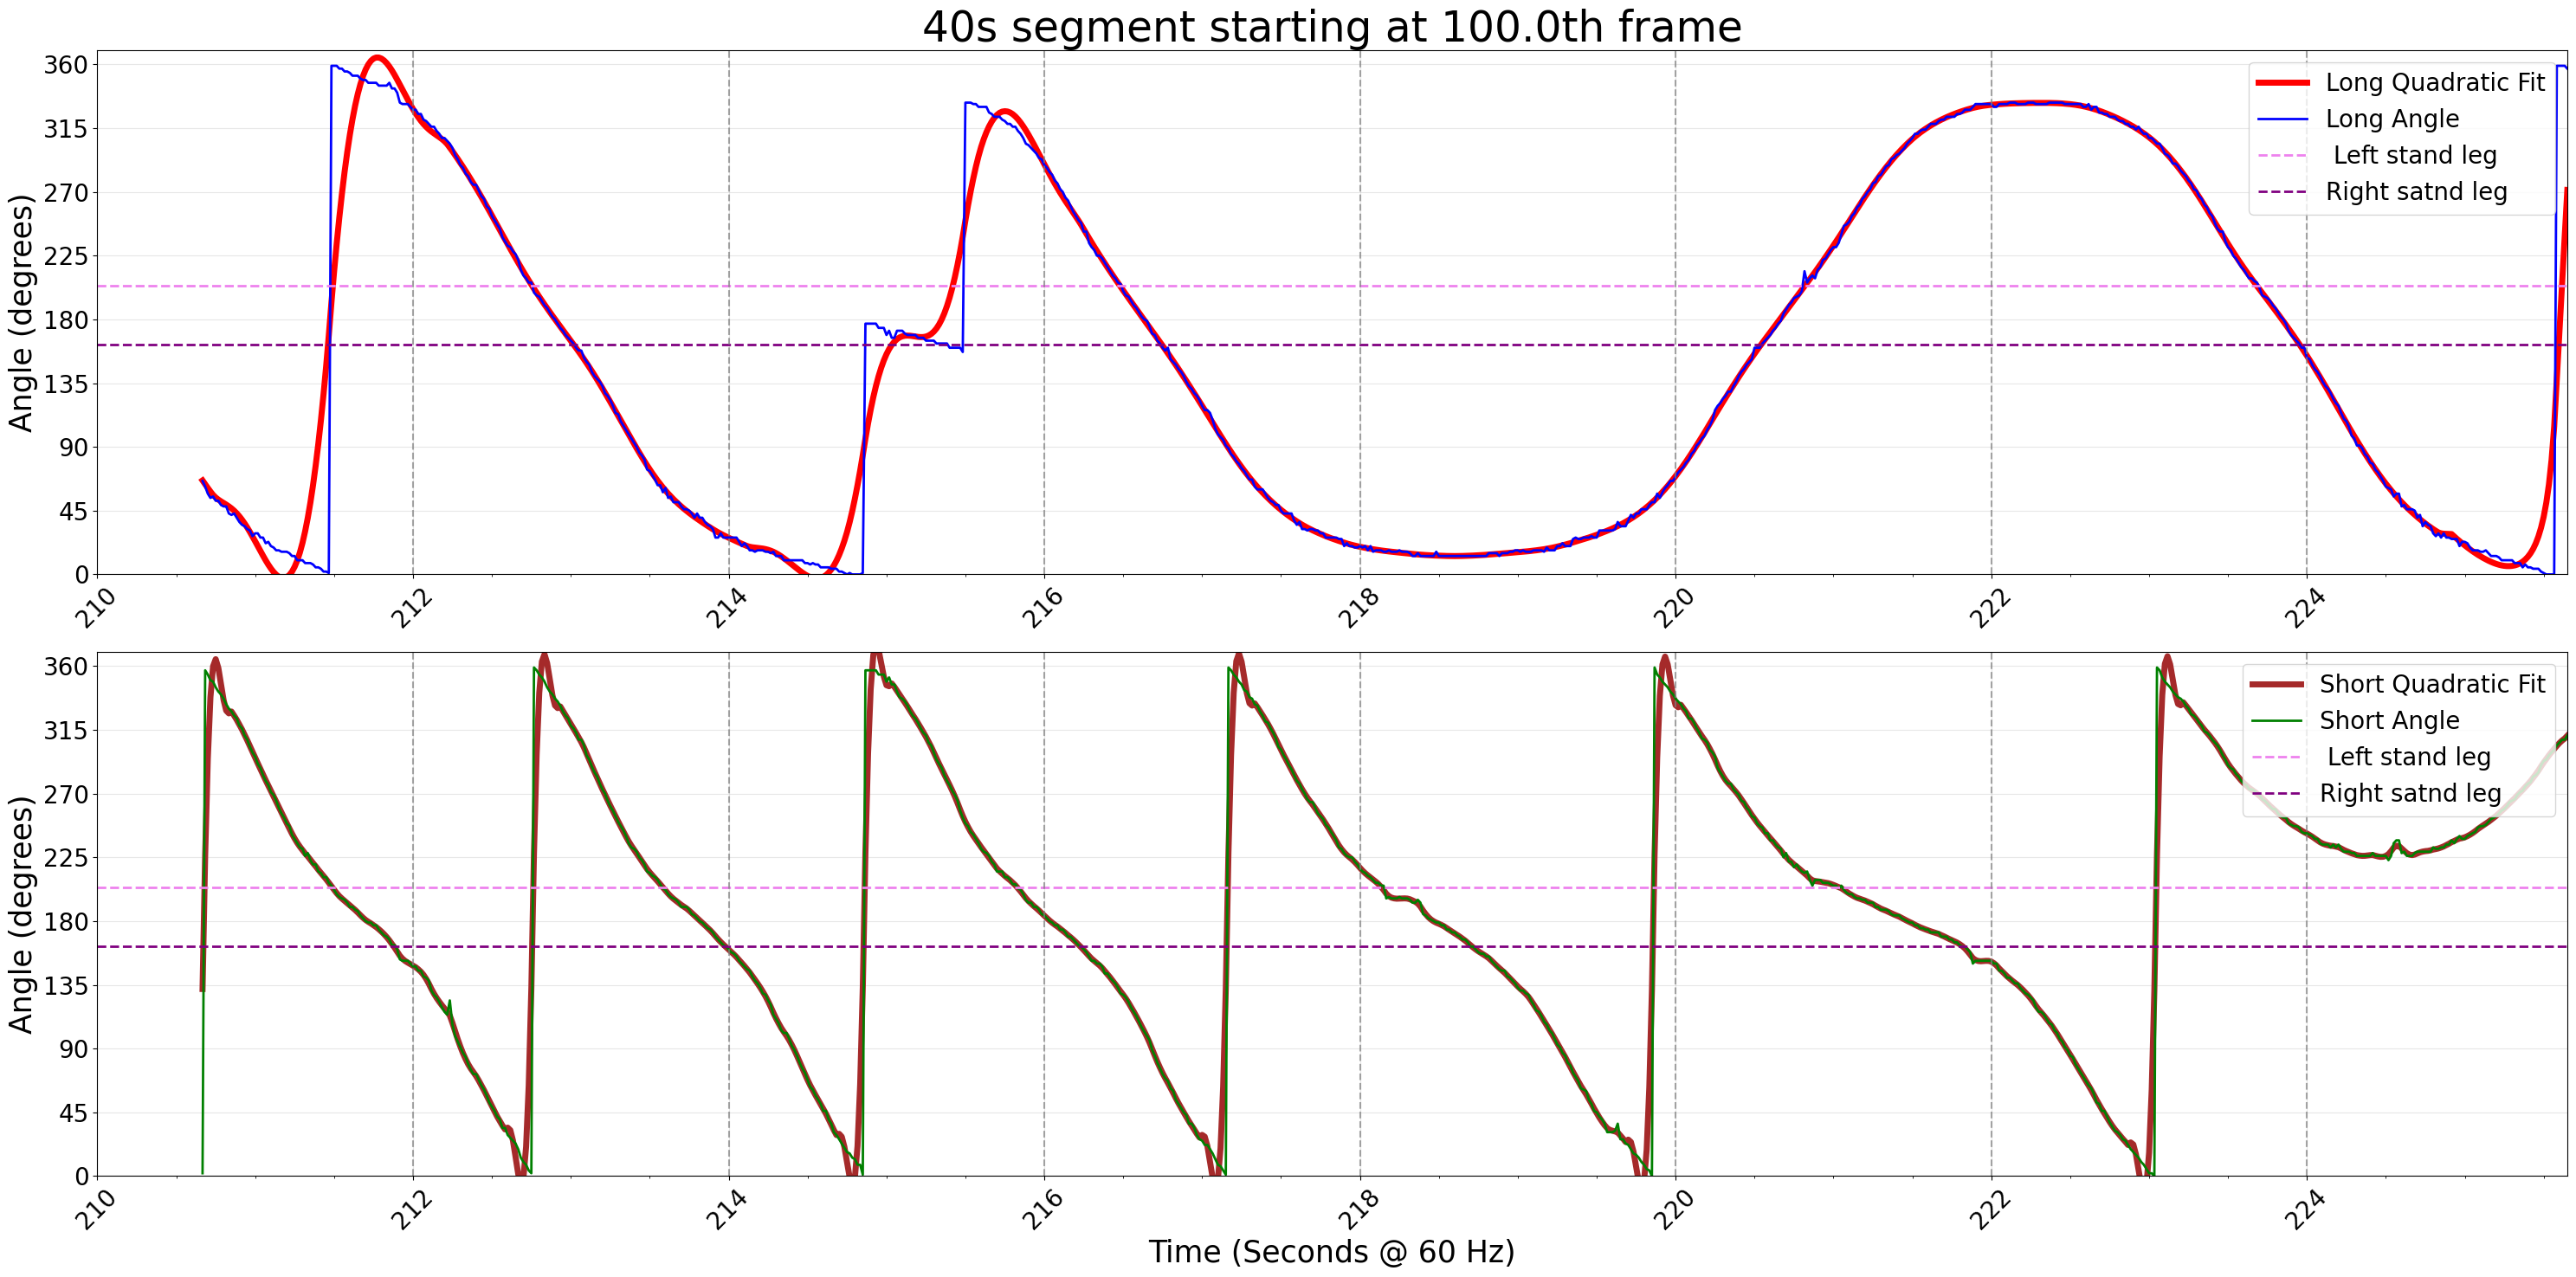
\includegraphics[width=1 \linewidth]{figures/long_short_sticks_raw_n_cleaned.png}
        %         \centering
        %         \caption{The graph on the top shows a section of raw(blue) and cleaned(red) of long stick timeseries. The bottom graph shows the raw(brown) and cleaned (green) timeseries of the short stick. The dotted lines on both graphs show the position of the left and right stands of the system}
        %         \label{fig:short_long_sticks_clean}
        % \end{figure}

        \newpage
       
        \section{Embedding and Feature Construction}
            In building set if supervised input vector and output forecast labels  for for over the top or next postion prediction, the choice of which feature is very important for characterize the best state or coordinate representation that is able to capture the dynamics of the kinetic swinging sticks motion. For forecasting, generally constructing the $X$ via Takens'
            delay embedding theorem with embedding dimension and delay determined empirically depending of the system being studied. However, the choice of input use for the delay embedding vectors affects the accuarcy of your forecast since they form or used as basis for determining the mapping of a state to it prediction next state.
            
            Fundamentally, obtaining a good model is linked to the coordinate system in which the dynamics are measured. Considering the state of the long or short stick is represented as an angle, forecasting the next state which is also an angle in degrees or radian, using Takens' delay embedding of timeseries is simple just as forecasting a time to the top, will required Taken embedding of over the top time positions to for $X$ used in building the mapping for each forecast.

            However, muitiple information in data presents different ways of building a training set data $X_L$ and $Y_L$; using  time, angle, angular velocity, time to over the top or change in time to over the top and clock hour positions.

            For whichever infrmation set used in building $X_L$  and $Y_L$, a model builds a map of using predicting target $y_t$ from $x_t$. For predictiion using local linear model at the core of method that leverages a kernel for determined weights used in 

             \subsection{Computing Distance in Delay Vectors of Angles}
                The first principles of a local linear model is selection of vectors that represent or characterize the 

            
       



    \section{Results}
        In this, we provide results obtained from baseline ablation study from  Echo State Networks (ESN), Support Vector Regression (SVR), Gaussian Process Regression or Bayesian (Probabilistic) (GPR), Multilayer Perceptron (MLP), Random Forest Regression (RF), Koopman operator(EDMD) and Long Short Term Memory (LSTM). For simpler prediction, we used the delay embedded vector angle representation.

        Three complementary metrics are reported:
            \begin{itemize}
              \item \textbf{RMSE}: $\sqrt{\frac{1}{N}\sum_i(y_i - \hat{y}_i)^2}$
              \item \textbf{NRMSE}: $\sqrt{\frac{\sum_i(y_i - \hat{y}_i)^2}{\sum_i(y_i - \bar{y})^2}}$
                      (variance-normalised; model is useful if NRMSE~$<1$)
              \item \textbf{{$R^2 (cod)$}}: $1 - \mathrm{NRMSE}^2$
              \item \textbf{MAE}: $\frac{1}{N}\sum_i|y_i - \hat{y}_i|$
            \end{itemize}

        \subsection{Ablation Protocol}
            For each model, we held all hyper-parameters at their default values
            and varied one hyperparameter at a time (\emph{one-at-a-time} or OAT
            ablation). This isolates the contribution of each parameter to the
            overall predictive performance. A full grid search is computationally
            intractable for all seven models jointly; OAT ablation provides directional
            sensitivity and is standard in reservoir computing
            literature~\cite{lukosevicius_reservoir_2009}.
        

        
        
        \subsection{Models Evaluation Table for Long and Short Sticks Ablation}
        Table~\ref{tab:summary} reports the test-set performance of each model
        with its best configuration identified during the ablation study.
        The GPR achieves the lowest NRMSE, consistent with its theoretical advantage
        as a probabilistic model with inherent memory matching the temporal structure
        of chaotic maps. GPR is competitive with ESN but is limited by its
        $\mathcal{O}(N^3)$ complexity (trained on $N=800$ samples here). SVR with
        RBF kernel performs well and offers strong practical guarantees via its
        convex optimization. MLP and RF are the most computationally efficient models
        and achieve competitive but slightly inferior NRMSE.
            

    % ===========================================================================
    \section{Conclusion}
        \label{sec:conclusion}
        % ===========================================================================


        We introduced an experimental dataset from the long-stick angle of the Swinging Sticks kinetic sculpture and performed a broad comparison of seven nonlinear time-series forecasters. Our ablation study on long sticks data, by systematically varying each model's key hyperparameters, showed that Bayesian kernel methods (GPR, NRMSE $= 0.00112$) and operator-theoretic
        approaches (EDMD, NRMSE $= 0.00620$) achieve the lowest normalized errors on one-step-ahead prediction. Simpler ensemble and feedforward models (RF, MLP) were nearly as accurate and substantially cheaper to train, while deep recurrent architectures (LSTM, NRMSE $= 0.15140$) were over-parameterised relative to the available data, incurring training times of 65--145\,s with no commensurate accuracy gain.

        For our short stick timeseries  forecast reveals an important shift in model ranking. SVR (NRMSE $= 0.02246$, $R^2 = 0.99950$), displaces GPR at the top, as the increased trajectory irregularity degrades the smoothness assumption underlying GPR's kernel. RF and EDMD remain competitive, while LSTM collapses ($R^2 = 0.65$), reinforcing that deep recurrent architectures are data-hungry relative to the available training set. Across both arms of the Swinging Sticks, kernel and ensemble methods prove the most reliable forecasters.
        
        
        In the future, we plan to leverage these findings in the system
        identification process as we attempt to infer interpretable governing
        equations of the Swinging Sticks. Since the underlying physics can be
        obtained analytically, data-driven methods such as SINDy or Koopman
        eigenfunctions may extract its dynamical equations directly from data.
        This work lays the groundwork by identifying the most promising learning
        models for capturing the chaotic dynamics of the Swinging Sticks system.


    
 \section*{ACKNOWLEDGMENT}
    %     The authors thank Dr.\ Leonard Smith for conceiving the study, composing the experimental design, initial analysis and
    %     invaluable feedback throughout this study. The authors also thank Dr.\ Creed Jones for his instruction and continued support. What's more, the authors gratefully acknowledge the resources and facilities provided by Virginia Tech.


    
    \section{Dataset and Code}
        The dataset and code used in this work are not publicly released during the review process to preserve the double-blind review policy and due to other restrictions. The authors will make the code and dataset available upon reasonable request and plan to release them publicly after acceptance.




\bibliographystyle{IEEEtran}
\bibliography{biblio}


% \appendix



\end{document}



